\ifx\wholebook\relax\else

% --------------------------------------------
% Lulu:

    \documentclass[a4paper,12pt,twoside]{../includes/ThesisStyle}

	\usepackage[T1]{fontenc} %%%key to get copy and paste for the code!
%\usepackage[utf8]{inputenc} %%% to support copy and paste with accents for frnehc stuff
\usepackage{times}
\usepackage{ifthen}
\usepackage{xspace}
\usepackage{alltt}
\usepackage{latexsym}
\usepackage{url}            
\usepackage{amssymb}
\usepackage{amsfonts}
\usepackage{amsmath}
\usepackage{stmaryrd}
\usepackage{enumerate}
\usepackage{cite}
%\usepackage[pdftex,colorlinks=true,pdfstartview=FitV,linkcolor=blue,citecolor=blue,urlcolor=blue]{hyperref}
\usepackage{xspace}
%\usepackage{graphicx}
\usepackage{subfigure}
\usepackage[scaled=0.85]{helvet}
        
        
\newcommand{\sepe}{\mbox{>>}}
\newcommand{\pack}[1]{\emph{#1}}
\newcommand{\ozo}{\textsc{oZone}\xspace}
\newcommand\currentissues{\par\smallskip\textbf{Current Issues -- }}

\newboolean{showcomments}
\setboolean{showcomments}{true}
\ifthenelse{\boolean{showcomments}}
  {\newcommand{\bnote}[2]{
	\fbox{\bfseries\sffamily\scriptsize#1}
    {\sf\small$\blacktriangleright$\textit{#2}$\blacktriangleleft$}
    % \marginpar{\fbox{\bfseries\sffamily#1}}
   }
   \newcommand{\cvsversion}{\emph{\scriptsize$-$Id: macros.tex,v 1.1.1.1 2007/02/28 13:43:36 bergel Exp $-$}}
  }
  {\newcommand{\bnote}[2]{}
   \newcommand{\cvsversion}{}
  } 


\newcommand{\here}{\bnote{***}{CONTINUE HERE}}
\newcommand{\nb}[1]{\bnote{NB}{#1}}
\newcommand{\fix}[1]{\bnote{FIX}{#1}}
%%%% add your own macros 

\newcommand{\sd}[1]{\bnote{Stef}{#1}}
\newcommand{\ja}[1]{\bnote{Jannik}{#1}}
\newcommand{\na}[1]{\bnote{Nico}{#1}}
%%% 


\newcommand{\figref}[1]{Figure~\ref{fig:#1}}
\newcommand{\figlabel}[1]{\label{fig:#1}}
\newcommand{\tabref}[1]{Table~\ref{tab:#1}}
\newcommand{\layout}[1]{#1}
\newcommand{\commented}[1]{}
\newcommand{\secref}[1]{Section \ref{sec:#1}}
\newcommand{\seclabel}[1]{\label{sec:#1}}

%\newcommand{\ct}[1]{\textsf{#1}}
\newcommand{\stCode}[1]{\textsf{#1}}
\newcommand{\stMethod}[1]{\textsf{#1}}
\newcommand{\sep}{\texttt{>>}\xspace}
\newcommand{\stAssoc}{\texttt{->}\xspace}

\newcommand{\stBar}{$\mid$}
\newcommand{\stSelector}{$\gg$}
\newcommand{\ret}{\^{}}
\newcommand{\msup}{$>$}
%\newcommand{\ret}{$\uparrow$\xspace}

\newcommand{\myparagraph}[1]{\noindent\textbf{#1.}}
\newcommand{\eg}{\emph{e.g.,}\xspace}
\newcommand{\ie}{\emph{i.e.,}\xspace}
\newcommand{\ct}[1]{{\textsf{#1}}\xspace}


\newenvironment{code}
    {\begin{alltt}\sffamily}
    {\end{alltt}\normalsize}

\newcommand{\defaultScale}{0.55}
\newcommand{\pic}[3]{
   \begin{figure}[h]
   \begin{center}
   \includegraphics[scale=\defaultScale]{#1}
   \caption{#2}
   \label{#3}
   \end{center}
   \end{figure}
}

\newcommand{\twocolumnpic}[3]{
   \begin{figure*}[!ht]
   \begin{center}
   \includegraphics[scale=\defaultScale]{#1}
   \caption{#2}
   \label{#3}
   \end{center}
   \end{figure*}}

\newcommand{\infe}{$<$}
\newcommand{\supe}{$\rightarrow$\xspace}
\newcommand{\di}{$\gg$\xspace}
\newcommand{\adhoc}{\textit{ad-hoc}\xspace}

\usepackage{url}            
\makeatletter
\def\url@leostyle{%
  \@ifundefined{selectfont}{\def\UrlFont{\sf}}{\def\UrlFont{\small\sffamily}}}
\makeatother
% Now actually use the newly defined style.
\urlstyle{leo}



	\usepackage{amsmath,amssymb}             % AMS Math
% \usepackage[french]{babel}
\usepackage[latin1]{inputenc}
\usepackage[T1]{fontenc}
\usepackage[left=1.5in,right=1.3in,top=1.1in,bottom=1.1in,includefoot,includehead,headheight=13.6pt]{geometry}
\renewcommand{\baselinestretch}{1.05}

\usepackage{multicol}

% Table of contents for each chapter

\usepackage[nottoc, notlof, notlot]{tocbibind}
\usepackage{minitoc}
\setcounter{minitocdepth}{1}
\mtcindent=15pt
% Use \minitoc where to put a table of contents

\usepackage{enumitem}

\usepackage{aecompl}

% Glossary / list of abbreviations

%\usepackage[intoc]{nomencl}
%\renewcommand{\nomname}{List of Abbreviations}
%
%\makenomenclature

% My pdf code

\usepackage[pdftex]{graphicx}
\usepackage[a4paper,pagebackref,hyperindex=true]{hyperref}

\usepackage{pgfplotstable,booktabs,colortbl}
\pgfplotsset{compat=1.8}

% Links in pdf
\usepackage{color}
\definecolor{linkcol}{rgb}{0,0,0.4} 
\definecolor{citecol}{rgb}{0.5,0,0} 

% Change this to change the informations included in the pdf file

% See hyperref documentation for information on those parameters

\hypersetup
{
bookmarksopen=true,
pdftitle="Sista: a Metacircular Architecture for Runtime Optimisation Persistence",
pdfauthor="Clement BERA", 
pdfsubject="Thesis", %subject of the document
%pdftoolbar=false, % toolbar hidden
pdfmenubar=true, %menubar shown
pdfhighlight=/O, %effect of clicking on a link
colorlinks=true, %couleurs sur les liens hypertextes
pdfpagemode=None, %aucun mode de page
pdfpagelayout=SinglePage, %ouverture en simple page
pdffitwindow=true, %pages ouvertes entierement dans toute la fenetre
linkcolor=linkcol, %couleur des liens hypertextes internes
citecolor=citecol, %couleur des liens pour les citations
urlcolor=linkcol %couleur des liens pour les url
}

% definitions.
% -------------------

\setcounter{secnumdepth}{3}
\setcounter{tocdepth}{1}

% Some useful commands and shortcut for maths:  partial derivative and stuff

\newcommand{\pd}[2]{\frac{\partial #1}{\partial #2}}
\def\abs{\operatorname{abs}}
\def\argmax{\operatornamewithlimits{arg\,max}}
\def\argmin{\operatornamewithlimits{arg\,min}}
\def\diag{\operatorname{Diag}}
\newcommand{\eqRef}[1]{(\ref{#1})}

\usepackage{rotating}                    % Sideways of figures & tables
%\usepackage{bibunits}
%\usepackage[sectionbib]{chapterbib}          % Cross-reference package (Natural BiB)
%\usepackage{natbib}                  % Put References at the end of each chapter
                                         % Do not put 'sectionbib' option here.
                                         % Sectionbib option in 'natbib' will do.
\usepackage{fancyhdr}                    % Fancy Header and Footer

% \usepackage{txfonts}                     % Public Times New Roman text & math font
  
%%% Fancy Header %%%%%%%%%%%%%%%%%%%%%%%%%%%%%%%%%%%%%%%%%%%%%%%%%%%%%%%%%%%%%%%%%%
% Fancy Header Style Options

\pagestyle{fancy}                       % Sets fancy header and footer
\fancyfoot{}                            % Delete current footer settings

%\renewcommand{\chaptermark}[1]{         % Lower Case Chapter marker style
%  \markboth{\chaptername\ \thechapter.\ #1}}{}} %

%\renewcommand{\sectionmark}[1]{         % Lower case Section marker style
%  \markright{\thesection.\ #1}}         %

\fancyhead[LE,RO]{\bfseries\thepage}    % Page number (boldface) in left on even
% pages and right on odd pages
\fancyhead[RE]{\bfseries\nouppercase{\leftmark}}      % Chapter in the right on even pages
\fancyhead[LO]{\bfseries\nouppercase{\rightmark}}     % Section in the left on odd pages

\let\headruleORIG\headrule
\renewcommand{\headrule}{\color{black} \headruleORIG}
\renewcommand{\headrulewidth}{1.0pt}
\usepackage{colortbl}
\arrayrulecolor{black}

\fancypagestyle{plain}{
  \fancyhead{}
  \fancyfoot{}
  \renewcommand{\headrulewidth}{0pt}
}

\usepackage{algorithm}
\usepackage[noend]{algorithmic}

%%% Clear Header %%%%%%%%%%%%%%%%%%%%%%%%%%%%%%%%%%%%%%%%%%%%%%%%%%%%%%%%%%%%%%%%%%
% Clear Header Style on the Last Empty Odd pages
\makeatletter

\def\cleardoublepage{\clearpage\if@twoside \ifodd\c@page\else%
  \hbox{}%
  \thispagestyle{empty}%              % Empty header styles
  \newpage%
  \if@twocolumn\hbox{}\newpage\fi\fi\fi}

\makeatother
 
%%%%%%%%%%%%%%%%%%%%%%%%%%%%%%%%%%%%%%%%%%%%%%%%%%%%%%%%%%%%%%%%%%%%%%%%%%%%%%% 
% Prints your review date and 'Draft Version' (From Josullvn, CS, CMU)
\newcommand{\reviewtimetoday}[2]{\special{!userdict begin
    /bop-hook{gsave 20 710 translate 45 rotate 0.8 setgray
      /Times-Roman findfont 12 scalefont setfont 0 0   moveto (#1) show
      0 -12 moveto (#2) show grestore}def end}}
% You can turn on or off this option.
% \reviewtimetoday{\today}{Draft Version}
%%%%%%%%%%%%%%%%%%%%%%%%%%%%%%%%%%%%%%%%%%%%%%%%%%%%%%%%%%%%%%%%%%%%%%%%%%%%%%% 

\newenvironment{maxime}[1]
{
\vspace*{0cm}
\hfill
\begin{minipage}{0.5\textwidth}%
%\rule[0.5ex]{\textwidth}{0.1mm}\\%
\hrulefill $\:$ {\bf #1}\\
%\vspace*{-0.25cm}
\it 
}%
{%

\hrulefill
\vspace*{0.5cm}%
\end{minipage}
}

\let\minitocORIG\minitoc
\renewcommand{\minitoc}{\minitocORIG \vspace{1.5em}}

\usepackage{multirow}
\usepackage{slashbox}

\newenvironment{bulletList}%
{ \begin{list}%
	{$\bullet$}%
	{\setlength{\labelwidth}{25pt}%
	 \setlength{\leftmargin}{30pt}%
	 \setlength{\itemsep}{\parsep}}}%
{ \end{list} }

\newtheorem{definition}{D�finition}
\renewcommand{\epsilon}{\varepsilon}

% centered page environment

\newenvironment{vcenterpage}
{\newpage\vspace*{\fill}\thispagestyle{empty}\renewcommand{\headrulewidth}{0pt}}
{\vspace*{\fill}}



	\graphicspath{{.}{../figures/}}
	\begin{document}
\fi

\chapter{Metacircular optimising JIT}
\label{chap:metacircular}
\minitoc

%Intro
By design, Scorch's optimiser and deoptimiser are written in Smalltalk and are running in the same runtime than the optimised application. This design leads to multiple problems similar to the ones existing in metacircular virtual machines. 

%single-threaded -> for comparison with Graal and co later
As Pharo is currently single-threaded, it is not possible to run Scorch in a concurrent native thread. To optimise code, Scorch requires either to temporarily interrupt the application green thread or to postpone the optimisation to a background-priority green thread as described in section \ref{sec:optModes}. The deoptimiser cannot however postpone the deoptimisation of a frame as it would block completely the running application. The deoptimiser has necessarily to interrupt the application green thread until deoptimisation is finished.

%introduction of the main issue
Hot spots can be detected in any Smalltalk code using conditionnal branches, including Scorch optimiser code itself (as Scorch is written in Smalltalk). When a hot spot is detected in the optimiser code, the optimiser interrupts itself and starts to optimise one of its own function. While doing so, the same hot spot may be detected again before any optimised function is installed, leading the optimiser to interrupt itself repeatedly. 

As Scorch deoptimiser is written in Smalltalk, its code base may get optimised. One of the optimisation-time speculation may be incorrect at runtime, leading the deoptimiser to require the deoptimisation of one of its own frame. In this case, the deoptimiser calls itself on one of its own frame, which may require to deoptimise a frame for the same function, leading the deoptimiser to call itself repeatedly. 

We call the \emph{infinite recursion} problem this issue where the optimiser or the deoptimiser respectively calls itself. The issue is detailed for each case in the first two sections.

%Different constraint so different solutions
The optimiser and deoptimiser have different constraints. It is possible to disable temporarily the optimiser while the application is running. In the worst case, a disabled optimiser leads to some functions not to be optimised, but the application keeps running correctly. However, the deoptimiser cannot be disabled temporarily while the application is running as the deoptimiser may be needed to keep executing code. As the optimiser and the deoptimiser have different constraints, they need different solutions for the infinite recursion problem.

%Outline and solution
This chapter explains the design used to avoid the infinite recursion issue in both the optimiser and the deoptimiser. The problem is solved in the optimiser by temporarily disabling it in specific circumstances. The deoptimiser solves the problem by using a code base completely independent from the rest of the system that cannot be optimised, hence it never requires to be deoptimised. The last section discuss similar design issues in other VMs and compares our solution to other solutions when relevant.

%%%%%%%%%%%%%%%%%%%%%%%%%%%%%%%%%%%%%%%%%%%%%%%%%%%%%%%%%%%%%%%%%%%%%%%%%%%%%%%%%%%%%%%%%%%%%%%%%%%%%%%%%%%%%%%%%%%%%%%%%%%%%

\section{Scorch optimiser}

%Intro, what Scorch optimiser does and critical mode.
Scorch optimiser is activated by the VM when a hot spot is detected. As Pharo is single-threaded, the optimiser is activated by interrupting the application green thread. The optimiser chooses, based on the current stack, a v-function to optimise.  Once the v-function to optimise is chosen, the optimiser gets started in critical mode: it attempts to generate an optimised v-function in a limited time period. If it succeeds, the optimised v-function is installed and used by further calls on the function. If the optimiser fails to generate the optimised v-function in the limited time period, it adds the v-function to a background compilation queue. In any case, the application is then resumed. When the application becomes idle, if the background compilation queue is not empty, Scorch gets activated in background mode. It produces and installs optimised v-functions for each function in the compilation queue without any time limit. 

\subsection{Infinite recursion issue}

%repeat problem for optimiser
As Scorch optimiser is written in Smalltalk, it can theoretically optimise its own code. In practice, if it happens, it may lead to an infinite recursion. Indeed, each time Scorch tries to optimise a function, before reaching the point where it can install the optimised function, it may interrupt itself to start optimising one of its own function. If a hot spot is detected in the optimiser code each time it attempts to optimise anything, then the optimiser never reaches the point where it can install an optimised function.

Figure \ref{fig:InfiniteRecursionOptPb} shows the problem. On the left, in the normal optimisation flow, the application is interrupted when a hot spot is detected, the optimiser generates an optimised v-function, installs it and the application resumes. On the right, in the infinite recursion issue, the application is also interrupted when a hot spot is detected, but while the optimiser is generating an optimised function, a hot spot is detected in the optimiser code. The optimiser then restarts to optimise one of its own function, but another hot spot is detected in the optimiser code. The optimiser keeps restarting the optimisation of one of its function.

\begin{figure}[h!]
    \begin{center}
        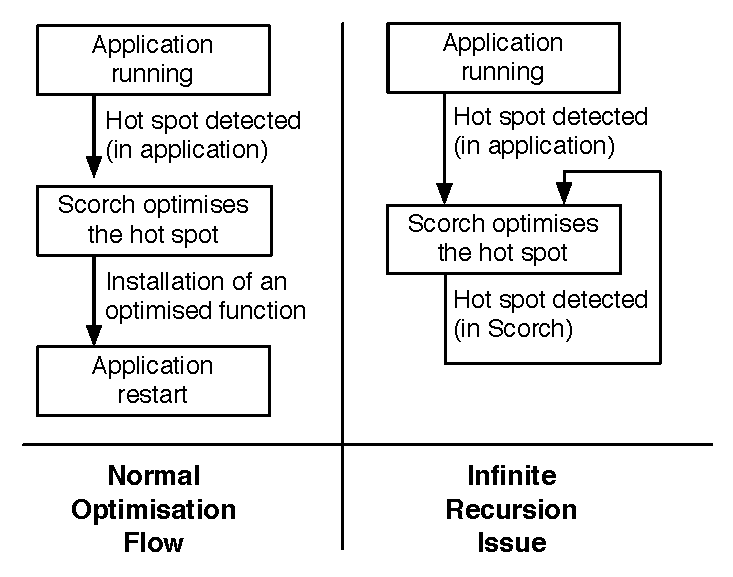
\includegraphics[width=0.65\linewidth]{InfiniteRecursionOptPb}
        \caption{Infinite recursion problem during optimisation}
        \label{fig:InfiniteRecursionOptPb}
    \end{center}
\end{figure}

In practice, the infinite recursion issue leads to a massive performance loss.

%slow down - critical
In critical mode, the optimiser has a limited time period to optimise code. If the infinite recursion issue happens, the optimiser spins until the time period ends as shown in figure \ref{fig:InfiniteRecursionOptPbCritical}. The application is then resumed without any optimised function installed. The application gets drastically slower as it gets interrupted for the full critical mode time period without gaining any performance from those interruptions.


\begin{figure}
    \begin{center}
		\subfigure[Critical mode]{\label{fig:InfiniteRecursionOptPbCritical}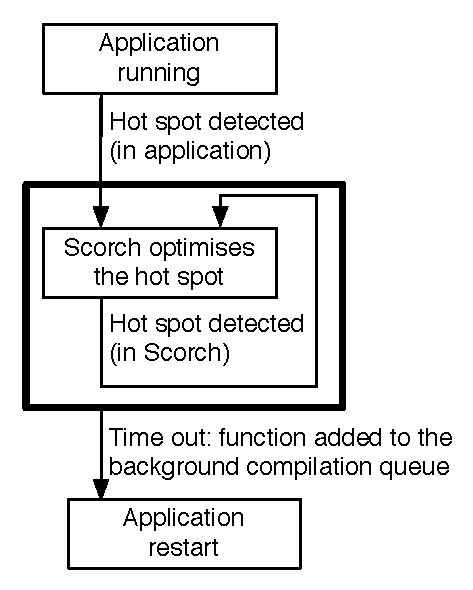
\includegraphics[width=0.4\linewidth]{InfiniteRecursionOptPbCritical}}
		\hfill
		\subfigure[Background mode]{\label{fig:InfiniteRecursionOptPbBackground}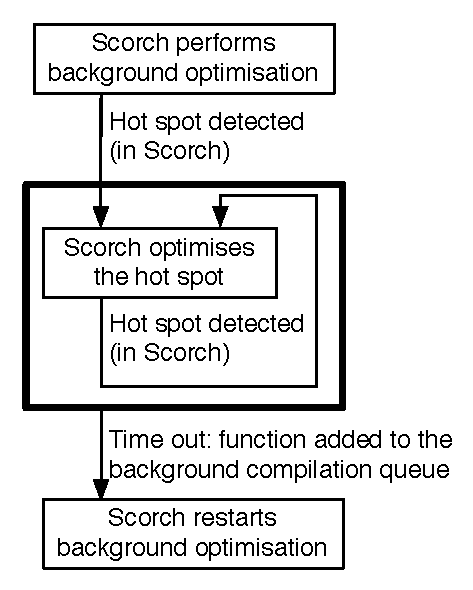
\includegraphics[width=0.4\linewidth]{InfiniteRecursionOptPbBackground}}
		\subfigure{
\includegraphics[width=0.3\linewidth]{InfiniteRecursionOptPbLegend}}
		\caption{Infinite recursion problem in the two optimisation modes}
    \end{center}
\end{figure}

%slow down - background
It can conceptually happen that the optimiser starts spinning while searching the stack for a function to optimise. In this case, no function can be added to the background compilation queue as the optimiser has not been able to find a function to optimise in the limited time period. In practice, in our case, the stack search code is quite simple and no hot spot can be detected repeatedly in this code.

When the application becomes idle, the optimiser is started in background mode to optimise functions in the background compilation queue. In this case, the optimiser always successfully generates and installs optimised functions. However, the optimisation of a function is verey slow. Indeed, while the optimiser is running in background mode, it activates itself in critical mode when detecting hot spots in its own code. Each time it happens, the optimiser spins in critical mode for the time period allowed as shown on figure \ref{fig:InfiniteRecursionOptPbBackground}. If the optimiser is started many times on itself during background optimisation, the optimisation of the function may take a significant amount of time. 

Eventually, the optimiser optimise most of its own code correctly through the background mode. Once done, both modes can work correctly as no hot spot can be detected in optimised code.

The problem is therefore that the application executed gets really slow at start-up because of time wasted spinning in critical mode. Peak performance takes a long time to reach because the optimiser successfully installs code only in background mode or when the infinite recursion issue does not happen in critical mode. 

\subsection{Current solution}

The first solution we wanted to implement was to disable the optimiser when it is running. This first design has a significant advantage: it is quite simple both conceptually and implementation-wise, while it completely avoids the infinite recursion problem. It has however a major drawback: the optimiser cannot optimise its own code any more. Of course, the optimiser may use core libraries that can be optimised. For example, the optimiser may use collections such as arrays. If the application optimised is also using the same collections, and it is very likely that an application would use arrays, the array code base may get optimised. Then, the optimiser ends up using an optimised version of arrays. For this reason, it is possible that while optimising code the optimiser triggers the deoptimiser, and it works perfectly fine.

%call-back removal / addition implementation
To implement our first solution, we changed the VM call-back activating the optimiser to uninstall itself upon activation. When a hot spot is detected but the call-back is not installed, the VM resets the profiling counters which has reached the hot spot threshold and restarts immediately the execution of the application. Then, we changed the optimiser to install back the call-back when it resumes the application, after adding a function to the background queue or installing optimised code. This way, we believed the optimiser would never end up in a situation where it optimises itself, solving entirely the problem.

%can optimise itself through back process
Then, we ran our benchmarks and saw that the problem was solved but the optimiser could still optimise its own code. Our first implementation effectively disabled the optimiser, but only when it was running on critical mode. When hot spots were detected, they were optimised or postponed without any issue as the optimiser disabled itself in critical mode, and the application resumed just fine. When the optimiser was started in background mode, it was not disabled. Hence, in this case, the optimiser was sometimes interrupted by itself in critical mode to get optimised.

%1st sol work and good enough 
This first solution is implemented, stable and works fine. Multiple benchmarks run with significant speed-up over the normal VM (This will be detailed in chapter \ref{chap:validation}). In general, in the production VM, simplicity is really important to keep the code base relatively easy to maintain. For each added complexity in the VM we wonder if the complexity is worth the benefit. This first solution is nice because it is simpler, both to understand and to maintain, than the alternative ones, so the optimising JIT may move to production with this design. Alternative solutions, more complex but with less constraints, are discussed in the next section.

\subsection{Discussion and advanced solutions}

%but cannot optimise itself in critical mode
The first solution is working but there is one major drawback: Scorch optimiser cannot optimise itself in critical mode. 

With the current solution, hot spots detected inside the optimiser in critical mode are completely ignored and the corresponding profiling counters are reset. If the optimiser attempts to inline code later, it may get confused by some counter values which were reset. The optimiser may speculate that a branch was not taken while in fact the branch was taken but the counters were reset. 

We could implement some kind of decay strategy instead of completely resetting the counters. We did not go in this direction because the counters are encoded in 16 bits while the hot spot threshold is at 60,000. Due to the 16 bits encoding limitation, not completely resetting the counters leads to many hot spot detected without anything happening, slowing down the optimiser code at start-up. Further analysis in this direction are required to conclude anything.

%the postpone pb while in critical mode - Saving current stack impossible
Based on advises from other people, we considered, instead of disabling the optimiser when it is running in critical mode, to postpone the optimisation to the background mode. In our design, it is quite difficult to do so. Indeed, when the VM call-back starts the optimiser, it provides only a reification of the current stack. The optimiser then needs to search the stack to select a function to optimise. As the stack is modified upon execution, it is not possible to save it efficiently so that the optimiser can search it later in the background green thread. As discussed in section \ref{ss:stackSearch}, there is no obvious cheap heuristic to figure out what function is the best to optimise based on the current stack (especially, picking the bottom frame function is usually not a good idea). It is however possible, once the optimiser has found what function to optimise, to add it to the background compilation queue. 

We believe that instead of disabling the entire optimiser while it is running in critical mode, we could instead disable it only during the stack searching phase in critical mode. The stack search phase represents less than 1\% of the optimiser execution time. The selected function optimisation may be postponed to the background green thread. This way, only hot spots detected during the stack search would be ignored, while the rest of the optimiser would be optimised at the next idle pause.

\paragraph{Ahead-of-time optimisation.} 
Alternatively, we could consider optimising the Scorch optimiser code ahead-of-time.

As the Sista architecture allows to persist optimised code (This is discussed in details in the following chapter), the optimiser code could be preheated through warm-up runs, for example by giving it a list of well-chosen functions to optimise. This way, all hot spots inside the optimiser would be detected ahead of time and optimised. The optimised optimiser code would be shipped to production.

Alternatively, the optimiser's code could be optimised statically by calling itself on its own code, using types inferred from a static type inferencer instead of types inferred from the runtime.

%\subsection{Dependencies and optimisations} 

% from 1 old part
%Rephrase -  solution does not forbig Scorch to use optimise libs

% maybe only one sentence ? -> be careful about dependencies
%The first constraint to note when programming Scorch, which may be obvious to the Kernel programmer, is that Scorch cannot depends on any framework or library but the Kernel and Core libraries. Each framework or library in the system relies on the execution engine to perform its code. Scorch is part of the execution engine. Hence, if Scorch relies on an external library and that someone modifies the library, the execution engine may not be stable any more and the runtime completely crashes. In fact, all the Kernel code and Core librairies have similar constraints, they cannot rely on anything to keep the system modular. 

%While writting Scorch, we needed a tool to compress the deoptimisation metadata generated aside from the optimised code. We wanted to use the standard Pharo serializer, Fuel (CITE), but we were not able to do it or further modification on Fuel would break the execution engine.

%In the end, we limited the dependencies of Scorch to the Pharo Kernel and the core collections (exactly: Set, OrderedCollection, Array, ByteArray and Dictionary in addition to the kernel). Any change on one of this dependency may require to change something in Scorch to keep the system running.


%\subsection{Debugging and runtime modification}

%Should I talk about that at all ? I was thinking over a restricted compiling to C but maybe we don't care.

%Maybe rewrite so that formally does not work but in practice it does.

%As any Smalltalk program, it is possible to modify the optimiser while it is running, for example in the debugger. If the modifications leads to incorrect optimiser behavior, then the runtime may crash. To avoid crashes, it may be wise to disable the optimiser while editing it. In practice, this feature is used only by the optimiser implementors. It is very useful to debug the optimiser to understand specific bugs or compiler decisions. With careful understanding of the infrastructure, it is possible in practice to debug the optimiser while it is running and modify its code. The optimiser is set by default to catch all exceptions, failing the optimisation of a specific v-function if an exception was raised. Hence, if the code modification triggers a compile-time exception, the system shall not crash. Unfortunately, in some cases, the optimiser may have silent errors, generating incorrect code without raising exceptions and completely crashing the system.

%The only part of Scorch that cannot really be edited is the deoptimisation metadata generation. Indeed, deoptimisation metadata is also used by the deoptimiser which, as detailled in the following section, has stronger constraints on its code. If one modifies the deoptimisation metadata generated, the deoptimiser may not be able to deoptimise correctly optimised code any more, leading to crashes.

%%%%%%%%%%%%%%%%%%%%%%%%%%%%%%%%%%%%%%%%%%%%%%%%%%%%%%%%%%%%%%%%%%%%%%%%%%%%%%%%%%%%%%%%%%%%%%%%%%%%%%%%%%%%%%%%%%%%%%%%%%%%%

%KEEP WRITING FROM HERE

\section{Scorch deoptimiser}

The deoptimiser can be activated in multiple contexts. If an optimisation time assumption is invalid at runtime, Cogit triggers a call-back to deoptimise the stack. Alternatively, multiple tools in the language, such as the debugging tools, may call the deoptimiser to introspect the stack.

\subsection{Infinite recursion issue}


%TODO repeat problem for deopt


On the contrary to the optimiser, deoptimisation cannot be postponed to a background green thread. The application green thread is blocked until the deoptimisation of the frame is performed. In addition, the deoptimiser cannot be disabled, or any application green thread requiring deoptimisation cannot continue executing code. The optimiser could be disabled as the execution could simply fall back to non optimised code. However, if the deoptimiser cannot restore the stack, the application green thread cannot keep executing code.

As the deoptimiser cannot be disabled, it is not possible to solve the infinite recursion problem in the same way than the optimiser. If the deoptimiser request deoptimisation, as for the optimiser requesting optimisation, the programs ends up in an infinite recursion where it keeps deoptimising / optimising itself. In the case of the optimiser, we could simply disable it while it is running, and the entire problem was solved. In the case of the deoptimiser, if we disable it and the deoptimiser request deoptimisation, the program cannot resume using non optimised code and crashes. 

To solve this infinite recursion problem, we implemented two solutions. The first solution attempts to restore the system in a recovery mode when recursive deoptimisation happens. It was used for the first benchmark, but it did not work correctly with benchmarks creating multiple green threads, and making it thread-safe had too many constraints. Then a second solution, used now, was designed and consists in keeping all the deoptimiser code in a library completely independent from the rest of the system that cannot be optimised.

\subsection{Recovery mode}

As a first attempt to solve the infinite recursion issue for the deoptimiser, we forced Scorch to keep a recovery copy of each method dictionary where optimised v-functions are installed. The recovery copies include only non optimised v-functions. We added a global flag, marking if a deoptimisation is in progress. If the deoptimiser is activated while a deoptimisation is in progress (this can be known thanks to the global flag), the deoptimiser falls back to recovery mode. Using the primitive \ct{become:}, the deoptimiser swaps all method dictionaries with their recovery copy and disables the optimiser. The deoptimiser can deoptimise the stack using only non optimised code. When the stack is deoptimised, the deoptimiser restores the method dictionaries with the optimised v-functions and re-enables the optimiser. 

Every function called from the deoptimisation call-back to the point where recovery mode is enabled cannot be optimised. We marked them with specific pragmas.

This approach worked for a while, but we had two major problems. 

The first problem is that switching to recovery mode requires to flush many caches in the VM to use the non optimised version of functions, and the caches need to be flushed again to switch back to optimised mode. As the infinite recursion issue is uncommon, one could argue that this problem may be acceptable. 

The second and main problem is that several of our benchmarks use multiple green threads. In this case, the global flag approach does not work as multiple deoptimisations may happen concurrently. In addition, the switches from recovery mode to optimised mode and the other way around needs to be wrapped in semaphores to be green thread safe. However, every function called from the deoptimisation cal-back to the point where recovery mode is enabled cannot be optimised. This now includes the semaphores and the process scheduler, and forbidding the optimisation of such code seemed to be too restrictive. We concluded that this approach could not work for our production environment.

\subsection{Independent library}

- completely independent and forbid deopt / opt

We could opt it statically.

Strong constraints: no dependency at all (duplicate array and dict), debugging is hardly possible.

Example of debugging -> can't log from deoptimiser. 

%%%%%%%%%%%%%%%%%%%%%%%%%%%%%%%%%%%%%%%%%%%%%%%%%%%%%%%%%%%%%%%%%%%%%%%%%%%%%%%%%%%%%%%%%%%%%%%%%%%%%%%%%%%%%%%%%%%%%%%%%%%%%

\section{Related work}

We find that stack search and deopt require specific rules. 

Implementing language --> problem only in Graal / metacircular VMs.

Thread system and our solution versus their solution.
implementing language like graal. single threaded. blabla.
However, compilation is done in same thread with hybrid interrupt / background approach
native threads - we are single threaded so that's how we do it.

solution of Graal, C++ for stack search and deopt while concurrent optimisation.

In Jalapeno, no deopt currently, profiling and optimisation concurrent 

%%%%%%%%%%%%%%%%%%%%%%%%%%%%%%%%%%%%%%%%%%%%%%%%%%%%%%%%%%%%%%%%%%%%%%%%%%%%%%%%%%%%%%%%%%%%%%%%%%%%%%%%%%%%%%%%%%%%%%%%%%%%%

\section{Conclusion}

In this chapter we discussed the main issue existing because the optimiser and the deoptimiser are implemented in Smalltalk and are running in the same runtime and the same native thread than the application they optimise and deoptimise respectively. The main issue is related to infinite recursion. If a hot spot is detected inside the optimiser code, the optimiser may call itself indefinitely to try to optimise it. The deoptimiser has a similar issue when it needs to deoptimise its own code. In both cases, the program may get slow or gets completely stuck.

The optimiser solves this issue by disabling itself when it runs in critical mode (when it interrupts temporarily the application green thread to perform the optimisation). The optimiser cannot optimise itself directly while running in critical mode, it can only optimise the  application, which may include libraries used both by the application and the optimiser itself. For functions taking a long time to optimise, the optimiser cannot stop the application for too long or the application becomes unresponsive, hence it postpone the optimisation to a background compilation queue where functions are optimised when the application is in idle. When performing optimisations in the background, the optimiser can optimise itself entirely.

The deoptimiser cannot solve the problem the same way as it cannot be disabled at any time or Smalltalk code cannot be executed any more. The deoptimiser avoids the problem by being written using a small number of classes that cannot be optimised nor call any other libraries.

\ifx\wholebook\relax\else
    \end{document}
\fi